\section{Calculus - Selected Topics}


\subsection{Problem 2.3}


\begin{figure}[!ht]
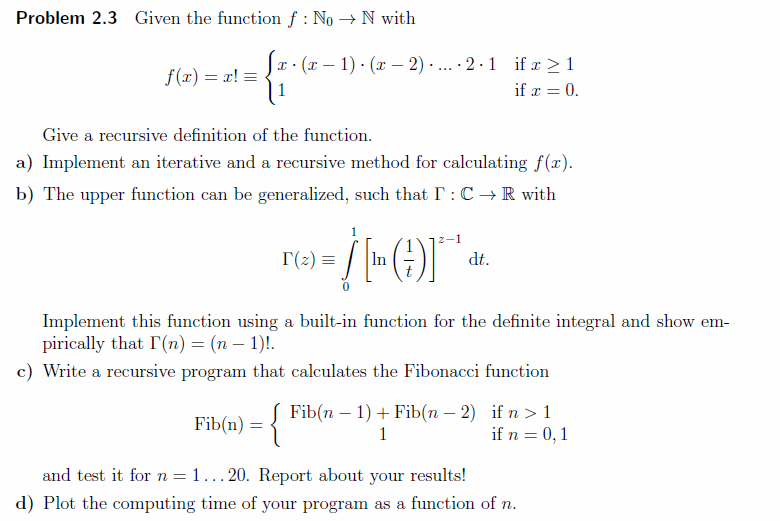
\includegraphics[width=1\textwidth]{chapters/images/desc-2-3}
\end{figure}


\subsubsection{a)}

X
\begin{lstlisting}[caption=todo]
n = int(input("n = "));

factorialIterative = 1;

for i in range(n):
    factorialIterative *= (i + 1);


print("iterative result: " + str(factorialIterative));

def factorialFunc(x):
    if x <= 0: return 1;
	
    return x * factorialFunc(x - 1);


factorialRecursive = factorialFunc(n);

print("recursive result: " + str(factorialRecursive));
\end{lstlisting}

results:

\begin{lstlisting}[caption=Result of 1.1 a), keywordstyle=\color{black}]
R
\end{lstlisting}

X



\subsubsection{b)}

X

\begin{lstlisting}[caption=todo]
import scipy.integrate as itg;

def bFunc(t, z):
	return math.pow(math.log(1 / t), z - 1);


for i in range(1, 10):
	factorialResult = factorialFunc(i - 1);
	integrateResult = itg.quad(lambda x: bFunc(x, i), 0, 1);
	
	print("n = " + str(i));
	print("(n - 1)! = " + str(factorialResult));
	print("Gamma(n) = " + str(integrateResult));

\end{lstlisting}


results:

\begin{lstlisting}[caption=Result of 1.1 a), keywordstyle=\color{black}]
R
\end{lstlisting}

X



\subsubsection{c)}

X

\begin{lstlisting}[caption=todo]

def fibonacciFunc(x):
	if x <= 1: return 1;
	
	return fibonacciFunc(x - 1) + fibonacciFunc(x - 2);


results = [];

for i in range(20):
	fib = fibonacciFunc(i);
	print("fib(" + str(i + 1) + ") = " + str(fib));
	results.append(fib);

\end{lstlisting}


results:

\begin{lstlisting}[caption=Result of 1.1 a), keywordstyle=\color{black}]
R
\end{lstlisting}

X



\subsubsection{d)}

X

\begin{lstlisting}[caption=todo]

runtimes = [];

for i in range(30):
	timeStart = time.time();
	fibonacciFunc(i);
	ms = 1000 * (time.time() - timeStart);
	runtimes.append(ms);


plt.plot(runtimes);
plt.xlabel('x');
plt.ylabel('runtime fib(x) [ms]');
plt.show();

\end{lstlisting}


results:



\begin{figure}[!ht]
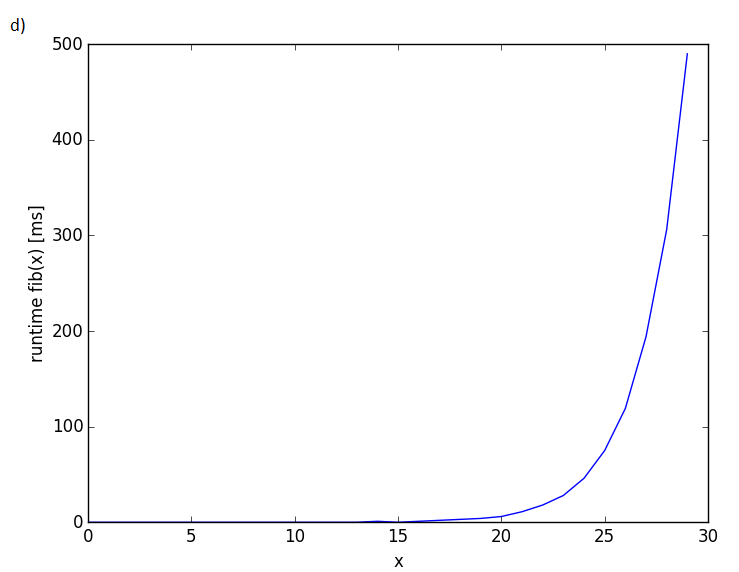
\includegraphics[width=1\textwidth]{chapters/images/figure-2-3-d}
\caption{todo}
\end{figure}







\subsection{Problem 2.4}


\begin{figure}[!ht]
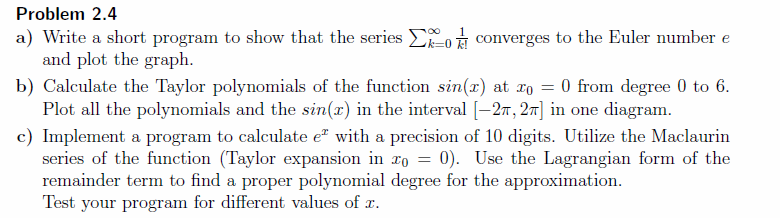
\includegraphics[width=1\textwidth]{chapters/images/desc-2-4}
\end{figure}


X

\begin{lstlisting}[caption=todo]

C

\end{lstlisting}

Y


\subsubsection{a)}

X

\begin{lstlisting}[caption=todo]

C

\end{lstlisting}


results:

\begin{lstlisting}[caption=Result of 1.1 a), keywordstyle=\color{black}]
R
\end{lstlisting}

X



\subsubsection{b)}

X

\begin{lstlisting}[caption=todo]

C

\end{lstlisting}


results:

\begin{lstlisting}[caption=Result of 1.1 a), keywordstyle=\color{black}]
R
\end{lstlisting}

X



\subsubsection{c)}

X

\begin{lstlisting}[caption=todo]

C

\end{lstlisting}


results:

\begin{lstlisting}[caption=Result of 1.1 a), keywordstyle=\color{black}]
R
\end{lstlisting}

X



\subsubsection{d)}

X

\begin{lstlisting}[caption=todo]

C

\end{lstlisting}


results:

\begin{lstlisting}[caption=Result of 1.1 a), keywordstyle=\color{black}]
R
\end{lstlisting}

X


\subsection{Problem 2.5}


\begin{figure}[!ht]
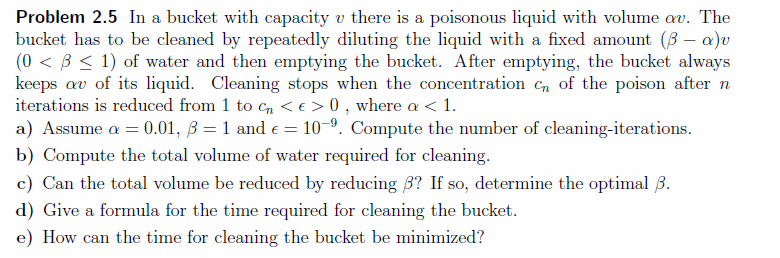
\includegraphics[width=1\textwidth]{chapters/images/desc-2-5}
\end{figure}


X

\begin{lstlisting}[caption=todo]

C

\end{lstlisting}

Y


\subsubsection{a)}

X

\begin{lstlisting}[caption=todo]

C

\end{lstlisting}


results:

\begin{lstlisting}[caption=Result of 1.1 a), keywordstyle=\color{black}]
R
\end{lstlisting}

X



\subsubsection{b)}

X

\begin{lstlisting}[caption=todo]

C

\end{lstlisting}


results:

\begin{lstlisting}[caption=Result of 1.1 a), keywordstyle=\color{black}]
R
\end{lstlisting}

X



\subsubsection{c)}

X

\begin{lstlisting}[caption=todo]

C

\end{lstlisting}


results:

\begin{lstlisting}[caption=Result of 1.1 a), keywordstyle=\color{black}]
R
\end{lstlisting}

X



\subsubsection{d)}

X

\begin{lstlisting}[caption=todo]

C

\end{lstlisting}


results:

\begin{lstlisting}[caption=Result of 1.1 a), keywordstyle=\color{black}]
R
\end{lstlisting}

X